% Options for packages loaded elsewhere
\PassOptionsToPackage{unicode}{hyperref}
\PassOptionsToPackage{hyphens}{url}
%
\documentclass[
]{article}
\usepackage{amsmath,amssymb}
\usepackage{iftex}
\ifPDFTeX
  \usepackage[T1]{fontenc}
  \usepackage[utf8]{inputenc}
  \usepackage{textcomp} % provide euro and other symbols
\else % if luatex or xetex
  \usepackage{unicode-math} % this also loads fontspec
  \defaultfontfeatures{Scale=MatchLowercase}
  \defaultfontfeatures[\rmfamily]{Ligatures=TeX,Scale=1}
\fi
\usepackage{lmodern}
\ifPDFTeX\else
  % xetex/luatex font selection
\fi
% Use upquote if available, for straight quotes in verbatim environments
\IfFileExists{upquote.sty}{\usepackage{upquote}}{}
\IfFileExists{microtype.sty}{% use microtype if available
  \usepackage[]{microtype}
  \UseMicrotypeSet[protrusion]{basicmath} % disable protrusion for tt fonts
}{}
\makeatletter
\@ifundefined{KOMAClassName}{% if non-KOMA class
  \IfFileExists{parskip.sty}{%
    \usepackage{parskip}
  }{% else
    \setlength{\parindent}{0pt}
    \setlength{\parskip}{6pt plus 2pt minus 1pt}}
}{% if KOMA class
  \KOMAoptions{parskip=half}}
\makeatother
\usepackage{xcolor}
\usepackage[margin=1in]{geometry}
\usepackage{graphicx}
\makeatletter
\def\maxwidth{\ifdim\Gin@nat@width>\linewidth\linewidth\else\Gin@nat@width\fi}
\def\maxheight{\ifdim\Gin@nat@height>\textheight\textheight\else\Gin@nat@height\fi}
\makeatother
% Scale images if necessary, so that they will not overflow the page
% margins by default, and it is still possible to overwrite the defaults
% using explicit options in \includegraphics[width, height, ...]{}
\setkeys{Gin}{width=\maxwidth,height=\maxheight,keepaspectratio}
% Set default figure placement to htbp
\makeatletter
\def\fps@figure{htbp}
\makeatother
\setlength{\emergencystretch}{3em} % prevent overfull lines
\providecommand{\tightlist}{%
  \setlength{\itemsep}{0pt}\setlength{\parskip}{0pt}}
\setcounter{secnumdepth}{-\maxdimen} % remove section numbering
\ifLuaTeX
  \usepackage{selnolig}  % disable illegal ligatures
\fi
\IfFileExists{bookmark.sty}{\usepackage{bookmark}}{\usepackage{hyperref}}
\IfFileExists{xurl.sty}{\usepackage{xurl}}{} % add URL line breaks if available
\urlstyle{same}
\hypersetup{
  pdftitle={Naive Bayes Classifier},
  pdfauthor={Emma},
  hidelinks,
  pdfcreator={LaTeX via pandoc}}

\title{Naive Bayes Classifier}
\author{Emma}
\date{}

\begin{document}
\maketitle

This is a group of machine learning algorithms which are used to
classify data. It's key features are that it \textbf{assumes
independence of predictors}, and gives \textbf{equal importance to each
predictor}.

It is based on Bayes theorem:

\[P(A|B) = \frac{P(B|A)P(A)}{P(B)}\]

Where A is the hypothesis and B is the predictors. For example, it might
calculate the \emph{probability of an email being spam (A)} given that
the email \emph{contains the text ``refund'' and it contains a link
(B)}. There are no interactions considered such as if an email is more
likely to contain a link if it contains ``refund''. Also, neither are
considered stronger indicators of the email being spam, both are given
equal importance.

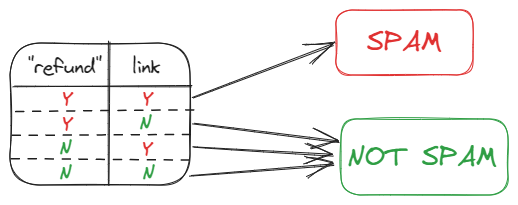
\includegraphics{spam_filter.png}

This type of algorithm is very simple so has a \textbf{low run time},
and can be effective with a \textbf{small training dataset}. It is
mainly used for \textbf{text classification} such as spam filtering or
sentiment analysis. One of the main weaknesses of this type of algorithm
is that real data is rarely independent which reduces performance of the
classifier. Some of its other weaknesses include that it is not a good
predictor so the probabilities given are not particularly accurate. It
also cannot learn which are the most important features to make
predictions.

\end{document}
